\newpage
\section{OOA-Klassenmodell}

Im Folgenden wird unser, auf Basis der Anforderungen unseres Planspiels,
erstelltes Klassendiagramm der Analysephase aus \ref{OOA-Client} und
\ref{OOA-Server} auf \pageref{OOA-Client} und \pageref{OOA-Server} n�her
erl�utert. 

Das Klassendiagramm ist in zwei H�lften aufgeteilt. In dem ersten Teil werden
die Klassen f�r den Clienten und die Klassen, die f�r die r�ndliche Kommunikation
zwischen Server und Client genutzt werden, abgebildet. Der zweite Teil enth�lt
die Klassen des Servers und Klassen und Interfaces, die f�r die
au�erordentliche Kommunikation zwischen Server und Client vorgesehen sind.

Das Herzst�ck des Unternehmens, dass auf Client-Seite vorgesehen ist, ist die
'Company' -Klasse. In ihr werden alle Entscheidungen des Spielers bearbeitet
und sie enth�lt alle Informationen, die der Spieler �ber sein Unternehmen
ben�tigt.
Dies sind die Mitarbeiter, die einzelnen Abteilungen und die Beziehungen, die zu
den einzelnen Regionen bestehen.

In den Beziehungen zu den Regionen werden entweder in einer 'ResourceRelation'
der Besitztum dieser Region erlangt und, sollte man schon eine solche Region
besitzen, auch die vorhandenen Geb�ude dieser Region gespeichert. Die
'CityRelation' enth�lt alle Informationen �ber die Bewohner einer Stadt und mit
dem 'Contract' auch �ber die Kunden des Unternehmens.

Die Abteilungen des Unternehmens umfassen das 'Warehouse', das
'InvestmentManagement', den 'Research', die 'Finances' und das 'Marketing'. In
dem Warehouse werden die Rohstoffe gelagert, die in Minen produziert
werden und die f�r die Produktion von Strom in den Kraftwerken ben�tigt werden.
Auch gehandelter Rohstoffe werden hier entnommen oder eingelagert.\\
Das InvestmentMangement beinhaltet alle Geb�ude (Minen und Kraftwerke) und alle
Grundst�cke (Regionen), die das Unternehmen besitzt. Hier werden neue Geb�ude
hinzugef�gt, Abschreibungen berechnet und Produktionsmengen eingestellt und
ausgelesen. Zudem besitzt jedes Kraftwerk mehrere 'PowerStationRelation', die
beinhaltet wieviel Energie das Kraftwerk den einzelnen, umliegenden St�dten
liefert. Diese Beziehung von einem Kraftwerk zu den St�dten ist vorgesehen,
damit die gewollte, maximale Lieferentfernung von drei Feldern nicht
�berschritten wird.\\
Die 'Finances' sind vorgesehen, um alle vier Quartale eine Bilanz und eine
Gewinn und Verlustrechnung aufzustellen. Alle Einnahmen und Ausgaben werden hier
eingespeichert und aufbereitet.\\
Das 'Marketing' ist vorgesehen um die Beliebtheit und die Bekanntheit
bei den Kunden zu beeinflussen.\\
Der letzte Bereich, der 'Research', ist vorgesehen um m�glicherweise eine aktive
Forschung einbauen zu k�nnen. Auf Grund von anderen Priorit�ten ist dieser aber 
nicht weiter modelliert und auch nicht in das entg�ltige Planspiel aufgenommen
worden.

Die Verbindung zwischen Client und Server wird aufgebaut indem sich der Client
�ber die 'Client'-Klasse mit der 'Server'-Klasse auf Serverseite verbindet. Dort
wird die Verbindung akzeptiert und nach dem 'Thread-per-Connection'-Prinzip ein,
f�r jeden Clienten seperater Thread der Klasse 'Connection' erstellt.

Die anschlie�ende Kommunikation wird mit Objekten, die jeweils das
'Messagable'-Interface implementieren durchgef�hrt. So kann jede beliebige
Klasse �bertragen werden. Der Empf�nger des Objektes kann nun den MessageType
des Objektes abfragen und wei� somit, wie er mit dem Objekt weiter verfahren
soll. Hierf�r sind spezielle Typen f�r jede unterschiedliche Nachricht, die
kommuniziert werden soll, in zwei Enumerates definiert.

�ber den Server werden jede Runde, alle Entscheidungen der Spieler abgewickelt,
die nicht nur den Spieler selbst, sondern auch andere Spieler betreffen. Vor
allem sind dies, Grundst�cksgebote und -k�ufe und Vertragseinstellungen mit
einer Stadt, nach denen die Kunden des Spielers bestimmt werden. Auch bereits
gebaute Geb�ude werden dem Server mitgeteilt, so dass sie f�r jeden Spieler
ersichtlich werden.

Diese �nderungen werden dem Clienten zu jedem Rundenbeginn �ber das
'Map'-Objekt und die 'CityRelation' mitgeteilt.

\begin{figure}
\centering
\centering
\hspace*{-30mm}
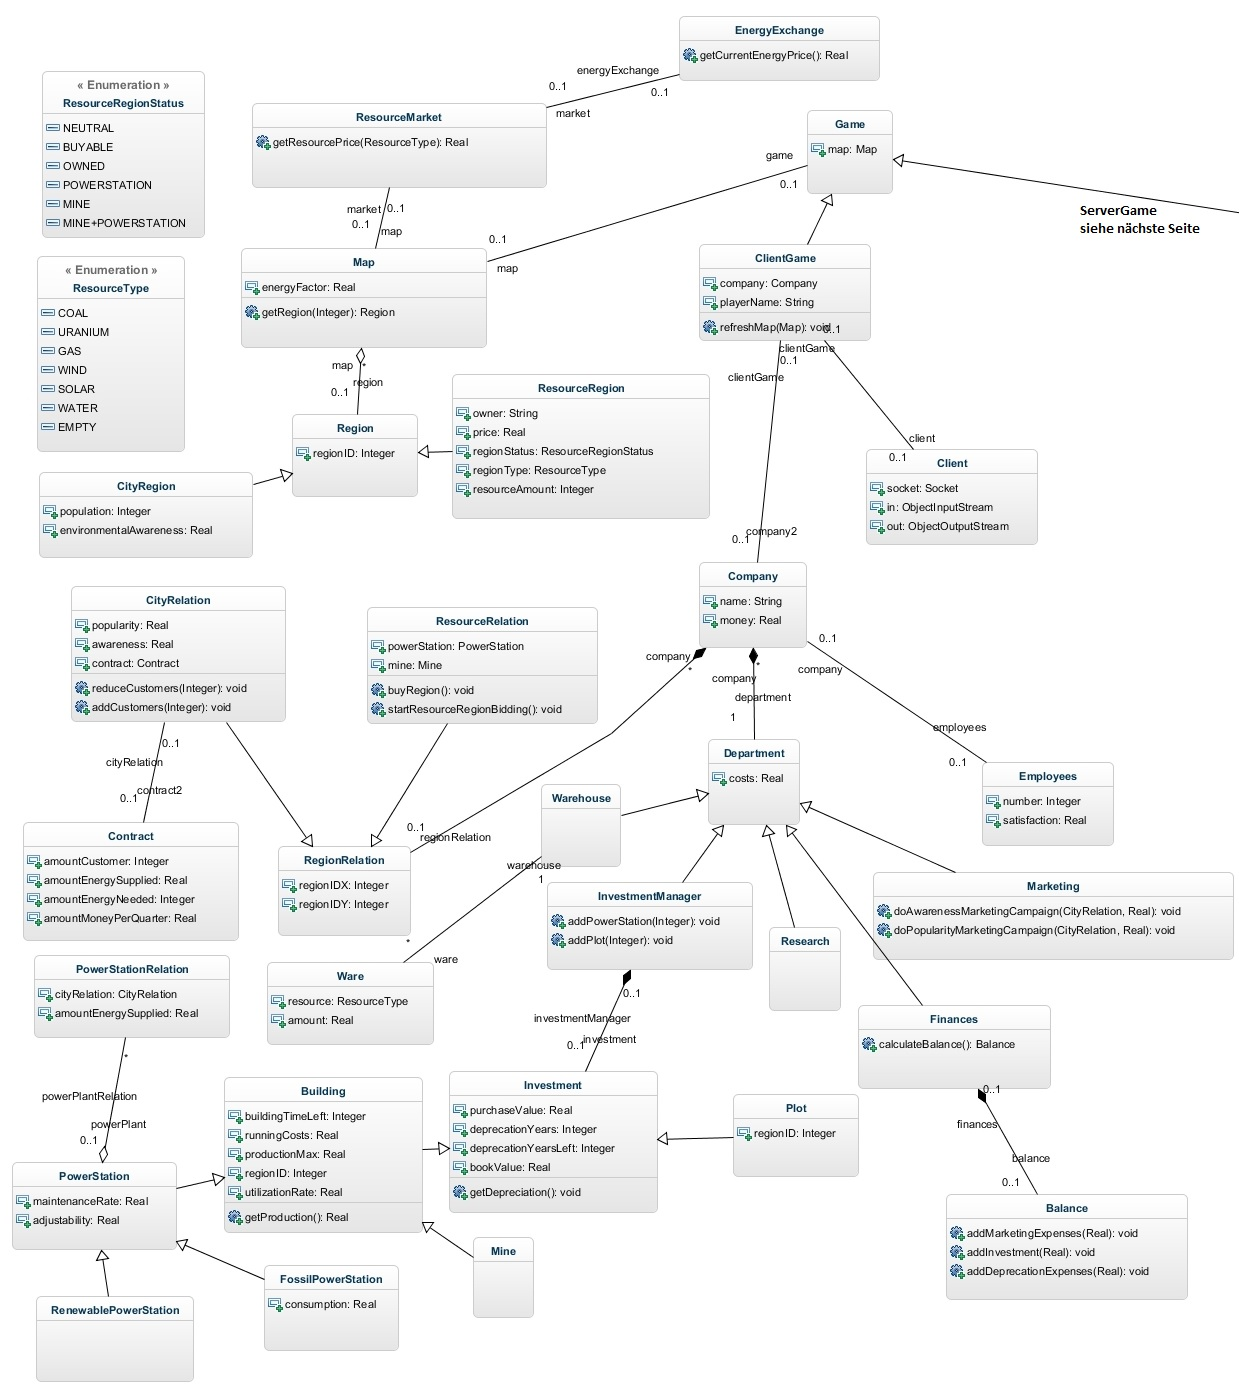
\includegraphics[width=1.3\textwidth]{se-wa-jpg/Client}
\caption{Klassendiagramm Teil 1}
\label{OOA-Client}
\end{figure}
%Die Grafik in Abbildung 
%\ref{labelname} auf Seite \pageref{labelname} ..
\begin{figure}
\centering
\centering
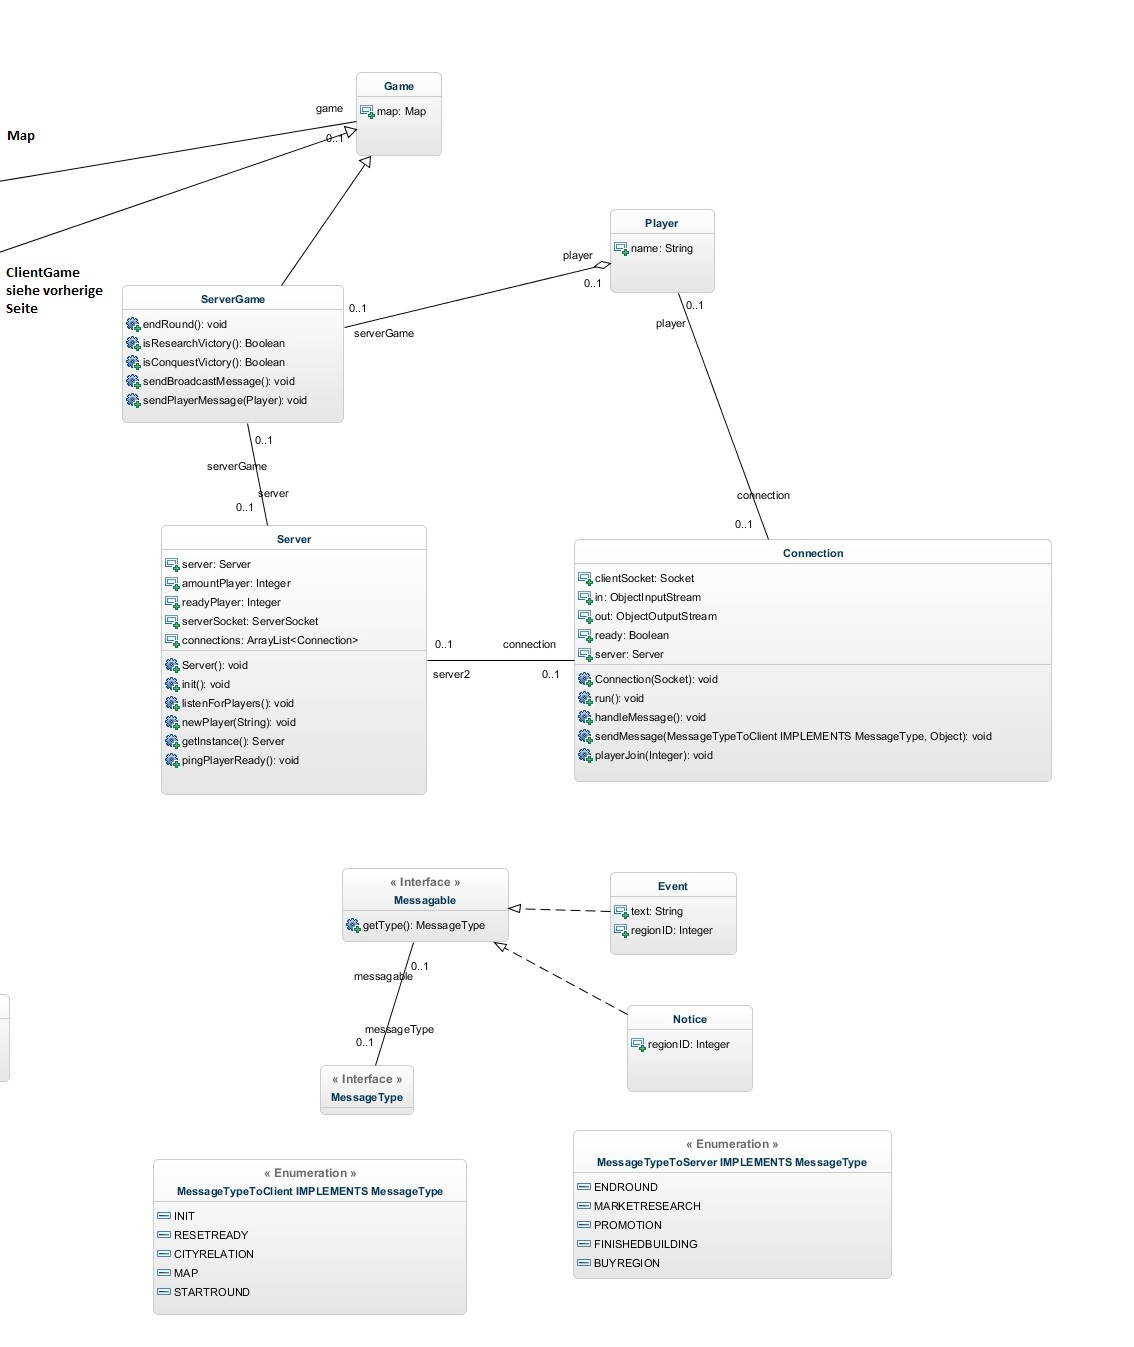
\includegraphics[width=1.1\textwidth]{se-wa-jpg/Server}
\caption{Klassendiagramm Teil 2}
\label{OOA-Server}
\end{figure}